% Copyright 2004 by Till Tantau <tantau@users.sourceforge.net>.
%
% In principle, this file can be redistributed and/or modified under
% the terms of the GNU Public License, version 2.
%
% However, this file is supposed to be a template to be modified
% for your own needs. For this reason, if you use this file as a
% template and not specifically distribute it as part of a another
% package/program, I grant the extra permission to freely copy and
% modify this file as you see fit and even to delete this copyright
% notice.

\documentclass[14pt]{beamer}

\usepackage{graphicx}

% There are many different themes available for Beamer. A comprehensive
% list with examples is given here:
% http://deic.uab.es/~iblanes/beamer_gallery/index_by_theme.html
% You can uncomment the themes below if you would like to use a different
% one:
%\usetheme{AnnArbor}
%\usetheme{Antibes}
%\usetheme{Bergen}
%\usetheme{Berkeley}
%\usetheme{Berlin}
%\usetheme{Boadilla}
%\usetheme{boxes}
%\usetheme{CambridgeUS}
%\usetheme{Copenhagen}
%\usetheme{Darmstadt}
%\usetheme{default}
%\usetheme{Frankfurt}
%\usetheme{Goettingen}
%\usetheme{Hannover}
%\usetheme{Ilmenau}
%\usetheme{JuanLesPins}
%\usetheme{Luebeck}
\usetheme{Madrid}
%\usetheme{Malmoe}
%\usetheme{Marburg}
%\usetheme{Montpellier}
%\usetheme{PaloAlto}
%\usetheme{Pittsburgh}
%\usetheme{Rochester}
%\usetheme{Singapore}
%\usetheme{Szeged}
%\usetheme{Warsaw}

\title{PEP-628}

% A subtitle is optional and this may be deleted
\subtitle{The world's oldest bug}

\author{@timl - Tim Leslie\inst{1}}
% - Give the names in the same order as the appear in the paper.
% - Use the \inst{?} command only if the authors have different
%   affiliation.

\institute[Breakaway Consulting] % (optional, but mostly needed)
{
  \inst{1}%
  Breakaway Consulting}
% - Use the \inst command only if there are several affiliations.
% - Keep it simple, no one is interested in your street address.

\date{PyCon AU, 2017}
% - Either use conference name or its abbreviation.
% - Not really informative to the audience, more for people (including
%   yourself) who are reading the slides online

\subject{Theoretical Computer Science}
% This is only inserted into the PDF information catalog. Can be left
% out.

% If you have a file called "university-logo-filename.xxx", where xxx
% is a graphic format that can be processed by latex or pdflatex,
% resp., then you can add a logo as follows:

% \pgfdeclareimage[height=0.5cm]{university-logo}{university-logo-filename}
% \logo{\pgfuseimage{university-logo}}

% Delete this, if you do not want the table of contents to pop up at
% the beginning of each subsection:
\AtBeginSubsection[]
{
  \begin{frame}<beamer>{Outline}
    \tableofcontents[currentsection,currentsubsection]
  \end{frame}
}

% Let's get started
\begin{document}

\begin{frame}
  \titlepage
\end{frame}

% Section and subsections will appear in the presentation overview
% and table of contents.
\section{First Main Section}

\begin{frame}{Two definitions of a circle}
    \begin{definition}
    A continuous set of points with a constant {\color{red}diameter}\\
    -- No-one (ever)
    \end{definition}
    \begin{definition}
    The set of all points a constant distance ({\color{red}radius}) from a center point\\
    -- Everyone (all the time)
    \end{definition}
\end{frame}

\begin{frame}{Constant Diameter - Not a circle}
\begin{center}
    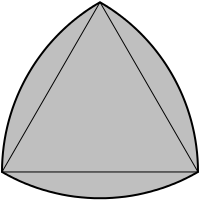
\includegraphics{ReuleauxTriangle}
\end{center}
\end{frame}

\begin{frame}{Definition of the circle constant}
\Large
\begin{equation*}
    \pi = \frac{\textrm{circumference}}{\textrm{diameter}}
\end{equation*}
  % You might wish to add the option [pausesections]
\end{frame}

\begin{frame}{Definition of the circle constant}
\Large
\begin{equation*}
    \pi = \frac{\textrm{circumference}}{\color{red}\textrm{diameter}}
\end{equation*}
\begin{center}
\newline
{\Huge This is a bug!}
\end{center}
  % You might wish to add the option [pausesections]
\end{frame}

\begin{frame}{Impacts of the bug}
\begin{center}
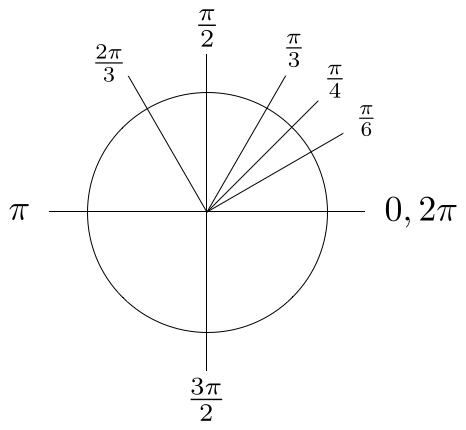
\includegraphics[height=5cm]{pi-angles}
\\$\pi$ represents half a circle
\end{center}
\end{frame}

\begin{frame}{Impacts of the bug}
\begin{center}
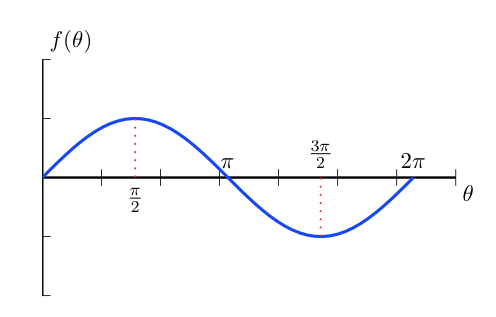
\includegraphics[height=5cm]{sine-wave}
\\$\pi$ represents half a period of a sine wave
\end{center}
\end{frame}

\begin{frame}{The workaround - $2\pi$}
\begin{equation*}
\frac{1}{\sqrt{\color{red}2\pi}\sigma}e^{-\frac{(x - \mu)^2}{2\sigma^2}}
\end{equation*}
\begin{equation*}
F(k) = \int_{-\infty}^{\infty}f(x)e^{-{\color{red}2\pi} i k x}\dx
\end{equation*}
\begin{equation*}
\zeta(2n) = \frac{B_n}{2(2n)!}({\color{red}2\pi})^{2n}
\end{equation*}
\end{frame}

\begin{frame}{The solution - tau ($\tau$)}
\huge
\begin{equation*}
\tau \equiv \frac{\textrm{circumference}}{\textrm{radius}} = 2\pi
\end{equation*}
\end{frame}

\begin{frame}{The solution - tau ($\tau$)}
\begin{center}
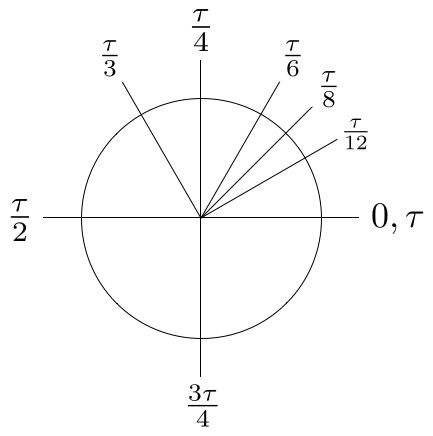
\includegraphics[height=5cm]{tau-angles}
\\$\tau$ represents a full circle
\end{center}
\end{frame}

\begin{frame}{The solution - tau ($\tau$)}
\begin{center}
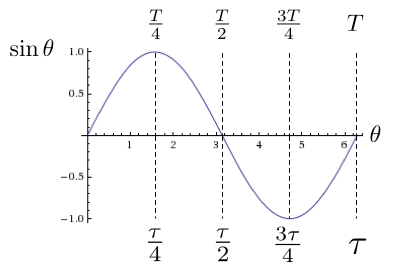
\includegraphics[height=5cm]{sine-with-tau}
\\$\tau$ represents a full period of a sine wave
\end{center}
\end{frame}

\begin{frame}{The solution - tau ($\tau$)}
\begin{equation*}
\frac{1}{\sqrt{\color{red}\tau}\sigma}e^{-\frac{(x - \mu)^2}{2\sigma^2}}
\end{equation*}
\begin{equation*}
F(k) = \int_{-\infty}^{\infty}f(x)e^{-{\color{red}\tau} i k x}\dx
\end{equation*}
\begin{equation*}
\zeta(2n) = \frac{B_n}{2(2n)!}{\color{red}\tau}^{2n}
\end{equation*}
\end{frame}

\begin{frame}{A bug in python}
\begin{block}{June, 2011, Nick Coghlan}
"We should add tau to the math module!" \\
PEP-628, issue12345
\end{block}
\begin{alertblock}{July, 2011, Guido}
"No"
\end{alertblock}
\end{frame}

\begin{frame}{Guido shares his benevolence}
\begin{block}{August, 2016, Guido}
"This PEP is now accepted and math.tau will be a part of Python 3.6.\\
Happy birtday Nick!"
\end{block}
\end{frame}

\begin{frame}{Victory}
\begin{center}
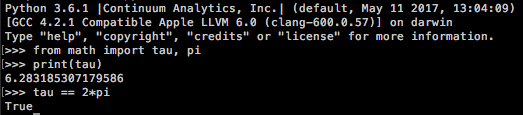
\includegraphics[width=12cm]{session}
\end{center}
\end{frame}

\begin{frame}{Further Reading}
\begin{itemize}
    \item \href{https://tauday.com/}{https://tauday.com/}
    \item \href{https://bugs.python.org/issue12345}{https://bugs.python.org/issue12345}
    \item \href{https://www.python.org/dev/peps/pep-0628/}{https://www.python.org/dev/peps/pep-0628/}
    \item @timl on twitter, pyconau.slack.com
\end{itemize}
\end{frame}

\end{document}
